
\documentclass{beamer}

\usetheme{CambridgeUS}
\usecolortheme{orchid}

\usepackage[utf8]{inputenc}
\usepackage[T1]{fontenc}

% Paths
\newcommand{\figs}{../figs}
\newcommand{\data}{../data}
\newcommand{\code}{../code}

% URL styles
\usepackage{url}
\urlstyle{sf}

% Units
\usepackage[detect-weight=true, binary-units=true]{siunitx}
\DeclareSIUnit\flop{Flops}

% Math
\usepackage{amsmath}
\usepackage{amssymb}
\usepackage{bm}
\usepackage{nicefrac}
\newcommand{\dif}[1]{{\;\text{d}#1}}

% Graphics
\usepackage{graphicx}
\usepackage{caption}
\usepackage{subcaption}
\graphicspath{{../figs/}}

% Tikz
\usepackage{tikz}
\usetikzlibrary{positioning,shapes,arrows,calc,intersections}
\usepackage{pgfplots}
\usepgfplotslibrary{dateplot}
\pgfplotsset{compat=1.8}

% Colors
\definecolor{darkblue}{HTML}{00688B}
\definecolor{darkgreen}{HTML}{6E8B3D}
\definecolor{cadet}{HTML}{DAE1FF}
\definecolor{salmon}{HTML}{FFB08A}

% Listings
\usepackage{textcomp}
\usepackage{listings}
\lstset{
  keywordstyle=\bfseries\color{orange},
  stringstyle=\color{darkblue!80},
  commentstyle=\color{darkblue!80},
  showstringspaces=false,
  basicstyle=\ttfamily,
  upquote=true,
}
\lstdefinestyle{fortran}{
  language=Fortran,
  morekeywords={for},
  deletekeywords={status},
}
\lstdefinestyle{c}{
  language=C,
  morekeywords={include},
}
\lstdefinestyle{glsl}{
  language=C,
  morekeywords={attribute, vec2, vec3, vec4, varying, uniform, mat2, mat3, mat4},
}
\lstdefinestyle{cuda}{
  language=C,
  morekeywords={__global__, __device__, __host__},
}
\lstdefinestyle{shell}{
  language=bash,
  morekeywords={mkdir, ssh, cmake},
}

% Double hlines
\usepackage{hhline}

% Misc
\usepackage{nth}

\subtitle{TMA4280---Introduction to Supercomputing}

\begin{document}


\title{Parallelization using OpenMP}
\author{Eivind Fonn}
\institute{SINTEF ICT / NTNU}
\date{December 2015}
\maketitle

\begin{frame}
  \frametitle{MPI - an overview}
  \begin{itemize}
  \item Several separate processes (separate instances) of the program.
  \item Processes communicate through message passing only.
  \item An MPI implementation requires substantial changes to the serial code.
  \item De-facto standard in the HPC community since the late eighties --- a
    consequence of the hardware available.
  \end{itemize}
\end{frame}

\begin{frame}
  \frametitle{Available hardware}
  \begin{itemize}
  \item In later years, even commodity processors now consist of several
    processing cores (the new ``kid in town'' to enable vendors to keep up with
    Moore's law).
  \item Two to four cores are the norm today.
  \item Vendors expect 8-16 cores to be the norm within a few years.
  \item This has resulted in an increased interest in shared-memory parallel
    programming libraries.
  \item HPC community also benefit from these developments.
  \item We here consider one such API; OpenMP.
  \end{itemize}
\end{frame}

\begin{frame}
  \frametitle{What is OpenMP?}
  \begin{itemize}
  \item OpenMP is a C/Fortran language extension for programming shared memory
    parallel machines.
  \item Implemented by most major vendors, e.g. Intel, IBM, SUN, as well as in
    open-source compilers, i.e., GNU/XCode as well as Microsoft Visual Studio
    (professional versions).
  \item The shared-memory programming model offers convenience and ease of
    implementation compared to a distributed memory model (MPI) when it can be
    used.
  \item However it also brings with it the challenges associated with sharing
    resources in multiple threads.
  \item Often combined with MPI on mixed distributed/shared memory machines
    (such as clusters and Vilje).
  \end{itemize}
\end{frame}

\begin{frame}
  \frametitle{Program flow in MPI}
  \begin{center}
    \scalebox{0.8}{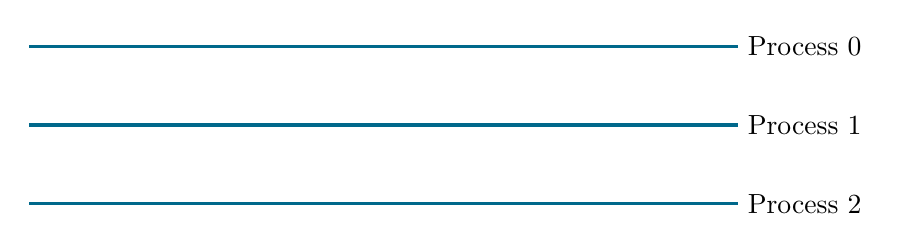
\begin{tikzpicture}
  \foreach \i in {0,...,2} {
    \draw[darkblue, very thick] (0,-\i) -- (9,-\i);
    \node[anchor=west] at (9,-\i) {Process \i};
  }
\end{tikzpicture}
}
  \end{center}
  \begin{itemize}
  \item In the MPI programming model, each processor has its own separate
    instance of the program.
  \item Hence we can consider the entire program to be one large parallel
    section of code.
  \item Typically parallelizing a program using MPI is done by first deciding on
    a data division between the processes, then dealing with the consequences of
    this division.
  \end{itemize}
\end{frame}

\begin{frame}
  \frametitle{Program flow in OpenMP}
  \begin{center}
    \scalebox{0.8}{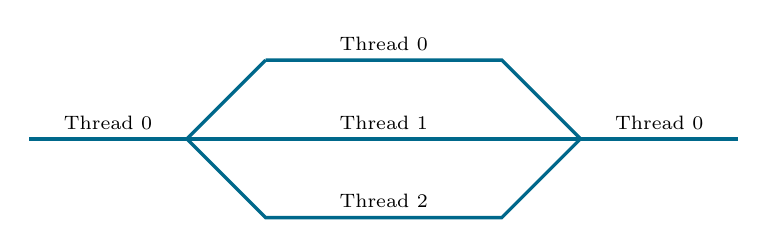
\begin{tikzpicture}
  \draw[darkblue, very thick] (0,0) -- (9,0);
  \draw[darkblue, very thick] (3,1) -- (6,1) -- (7,0) -- (6,-1) -- (3,-1) -- (2,0) -- (3,1);
  \node[anchor=south] at (8,0) {\scriptsize Thread 0};
  \node[anchor=south] at (1,0) {\scriptsize Thread 0};
  \node[anchor=south] at (4.5,1) {\scriptsize Thread 0};
  \node[anchor=south] at (4.5,0) {\scriptsize Thread 1};
  \node[anchor=south] at (4.5,-1) {\scriptsize Thread 2};
\end{tikzpicture}
}
  \end{center}
  \begin{itemize}
  \item OpenMP however, is based on a fork-join programming model.
  \item We only have one process.
  \item The main program flow happens on one processor.
  \item In sections we mark as parallel using \texttt{\#pragma}'s, the program
    flow forks into separate threads which run in parallel. Once we leave the
    parallel section, the program flow is returned to the main thread.
  \item No explicit data division is performed.
  \end{itemize}
\end{frame}

\begin{frame}
  \frametitle{Operations suitable for OpenMP}
  \begin{itemize}
  \item Moderately large computation intensive operations. Since
    thread-dispatchment always has some costs attached, spawning multiple
    threads easily costs more time than what you gain by doing the calculations
    in parallel if the operations are too small.
  \item Decoupled problems. Since the threads are sharing resources, we have to
    protect resources using mutual exclusion locks if several threads need to
    read/write to the same resources concurrently. This adds code complexity and
    in most cases severe loss of performance. OpenMP shines when you are able to
    decouple problems in large, independent chunks.
  \end{itemize}
\end{frame}

\begin{frame}
  \frametitle{How to use OpenMP}
  \begin{itemize}
  \item OpenMP is used by giving the compiler instructions through
    \texttt{\#pragma} commands. Note that these instructions are \emph{NOT} part
    of the programming language itself, in contrast to \texttt{MPI}.
  \item There are two types of pragmes: those used in combination with loop
    constructs, or those that are used to mark sections of the code that can run
    in parallel.
  \end{itemize}
\end{frame}

\begin{frame}[fragile]
  \frametitle{Example: loop with fixed cost}
  \begin{lstlisting}[style=c]
    for (int i = 0; i < 100; i++)
      do_something(i);
  \end{lstlisting}
  \begin{itemize}
  \item We assume that \texttt{do\_something} does not depend on any global
    resources: each call is independent of any other call.
  \item To split this loop among several threads, you can simply do
    \begin{lstlisting}[style=c]
#pragma omp parallel for schedule(static)
for (int i = 0; i < 100; i++)
  do_something(i);
    \end{lstlisting}
  \end{itemize}
\end{frame}

\begin{frame}[fragile]
  \frametitle{Example: loop with fixed cost}
  \begin{lstlisting}[style=c]
    #pragma omp parallel for schedule(static)
  \end{lstlisting}
  The pragma has three parts:
  \begin{itemize}
  \item \texttt{\#pragma omp}: all OpenMP directives start with this.
  \item \texttt{parallel for}: tells the compiler that the following for-loop
    should be parallelized.
  \item \texttt{schedule(static)}: tells the compiler to give each thread
    approximately the same number of iterations up-front.
  \end{itemize}
\end{frame}

\begin{frame}[fragile]
  \frametitle{Example: loop with varying cost}
  If each call to \texttt{do\_something(i)} may take a different amount of time,
  depending perhaps on \texttt{i}, we can use dynamic scheduling:
  \begin{lstlisting}[style=c]
    #pragma omp parallel for schedule(dynamic)
    for (int i = 0; i < 100; i++)
      do_something(i);
  \end{lstlisting}
  This instructs the compiler not to divide the work up-front, but instead leave
  one thread as a ``broker''. Initially, each thread is assigned a single
  iteration. Upon completing this, they ask the broker for more work. The broker
  keeps handing out work until each iteration has been assigned.
\end{frame}

\begin{frame}[fragile]
  \frametitle{Example: loop with varying cost}
  \begin{itemize}
  \item This works well if there are many iterations, and each of them are
    suitably expensive.
  \item If the iterations are cheap, then execution time will be dominated by
    negotiating with the broker thread, since this can only happen serially.
  \item We can minimize this problem by specifying a \emph{chunk size},
  \begin{lstlisting}[style=c]
#pragma omp parallel for schedule(dynamic, 5)
for (int i = 0; i < 100; i++)
  do_something(i);
  \end{lstlisting}
  \item Now, the broker hands out assignments in chunks of five. Each chunk is
    now expensive enough that the broker is not overrun.
  \end{itemize}
\end{frame}

\begin{frame}[fragile]
  \frametitle{Example: loop with varying cost}
  \begin{itemize}
  \item By using a fixed chunk size, we may end up in a situation where all the
    remaining work is assigned to a single thread. (Poor load balancing.)
  \item OpenMP offers a third scheduling mode to help fix this problem.
  \begin{lstlisting}[style=c]
#pragma omp parallel for schedule(guided, 5)
for (int i = 0; i < 100; i++)
  do_something(i);
  \end{lstlisting}
  \end{itemize}
\end{frame}

\begin{frame}[fragile]
  \frametitle{Example: sections}
  Consider the serial snippet
  \begin{lstlisting}[style=c]
    do_job_1();
    do_job_2();
    do_job_3();
  \end{lstlisting}
  Again we assume that the jobs are independent and share no resources, but they
  are different enough in nature that it doesn't make sense to write this in the
  form of a loop.
\end{frame}

\begin{frame}[fragile]
  \frametitle{Example: sections}
  This can be parallelized as such.
  \begin{lstlisting}[style=c, basicstyle=\ttfamily\footnotesize]
    #pragma omp parallel sections
    {
      #pragma omp parallel section
      {
        do_job_1();
      }
      #pragma omp parallel section
      {
        do_job_2();
      }
      #pragma omp parallel section
      {
        do_job_3();
      }
    }
  \end{lstlisting}
\end{frame}

\begin{frame}[fragile]
  \frametitle{Critical sections}
  \begin{center}
    \scalebox{0.8}{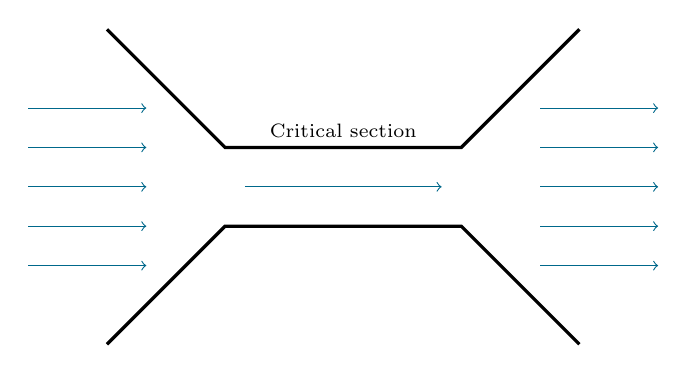
\begin{tikzpicture}[scale=0.5]
  \draw[very thick] (-6,4) -- (-3,1) -- (3,1) -- (6,4);
  \draw[very thick] (-6,-4) -- (-3,-1) -- (3,-1) -- (6,-4);
  \draw[darkblue, ->] (-2.5,0) -- (2.5,0);
  \foreach \i in {-2,...,2} {
    \draw[darkblue, ->] (-8,\i) -- (-5,\i);
    \draw[darkblue, ->] (5,\i) -- (8,\i);
  }
  \node[anchor=south] at (0,1) {\scriptsize Critical section};
\end{tikzpicture}
}
  \end{center}
  A critical section is a part of the code that, for whatever reason, should
  only be accessed by one thread at a time. Typically this happens whenever you
  need to read or write from or to shared resources.
\end{frame}

\begin{frame}[fragile]
  \frametitle{Critical sections: explicit locks}
  You can use mutexes (\emph{mutual exclusion locks}) for this.
  \begin{lstlisting}[style=c]
    omp_lock_t my_lock;
    omp_init_lock(&my_lock);

    #pragma omp parallel for
    for (int i = 0; i < 100; i++) {
      do_something(i);

      omp_set_lock(&my_lock);
      // critical section
      omp_unset_lock(&my_lock);
    }

    omp_destroy_lock(&my_lock);
  \end{lstlisting}
\end{frame}

\begin{frame}[fragile]
  \frametitle{Critical sections: pragmas}
  OpenMP has built-in language support for critical sections.
  \begin{lstlisting}[style=c]
    #pragma omp parallel for
    for (int i = 0; i < 100; i++) {
      do_something(i);

      #pragma omp critical
      {
        // critical section
      }
    }
  \end{lstlisting}
\end{frame}

\begin{frame}[fragile]
  \frametitle{Critical sections: pragmas}
  You can even have named critical sections.
  \begin{lstlisting}[style=c, basicstyle=\ttfamily\footnotesize]
    #pragma omp parallel for
    for (int i = 0; i < 100; i++) {
      do_something(i);

      #pragma omp critical updateLog
      {
        // update the log file
      }

      do_something_else(i);

      #pragma omp critical updateLog
      {
        // update the log file
      }
    }
  \end{lstlisting}
\end{frame}

\begin{frame}[fragile]
  \frametitle{How to enable}
  \begin{itemize}
  \item With GNU compilers (\texttt{gcc}, \texttt{g++}, \texttt{gfortran}), use
    the compiler flag \texttt{-fopenmp}.
  \item With Intel compilers (\texttt{icc}, \texttt{icpc}, \texttt{ifort}), use
    the compiler flag \texttt{-openmp}.
  \item Without this flag, GNU compilers will silently ignore pragmas, while
    Intel compilers will give a warning. In either case, the resulting binary is
    equivalent to serial code.
  \item In CMake you can do this
    \begin{lstlisting}[basicstyle=\ttfamily\footnotesize]
find_package(OpenMP)
if(OPENMP_FOUND)
  set(CMAKE_C_FLAGS
      "${CMAKE_C_FLAGS} ${OpenMP_C_FLAGS}$")
endif()
    \end{lstlisting}
%$
  \end{itemize}
\end{frame}

\begin{frame}
  \frametitle{Conclusions}
  \begin{itemize}
  \item OpenMP offers easy exploitation of computing resources on shared memory
    machines.
  \item The parallel code is very close to the serial code - it usually only
    differs by some pragmas which you can tell a compiler to ignore.
  \item The fork-join programming model often is harder to grasp than the
    distributed model, in particular if several threads need to access the same
    resources.
  \item Best results are usually achieved if you combine OpenMP and MPI. This is
    also the model that maps the best to modern hardware, where you typically
    have a few handfuls of CPUs sharing memory, while using more than that
    requires a distributed memory programming model.
  \end{itemize}
\end{frame}

\begin{frame}
  \frametitle{More information}
  \begin{center}
    The official page for the OpenMP specification can be found at \\~\\
    http://openmp.org \\~\\~\\~\\
    Some very instructive tutorials can be found at \\~\\
    http://computing.llnl.gov/tutorials/openMP
  \end{center}
\end{frame}

\end{document}

